\documentclass[11pt]{article}

\usepackage[utf8]{inputenc}
\usepackage[T1]{fontenc}
\usepackage[ngerman]{babel}


\usepackage[margin=1in]{geometry}		% For setting margins
\usepackage{amsmath}				% For Math
\usepackage{siunitx}
\usepackage{multicol}
\usepackage{fancyhdr}% For fancy header/footer

\usepackage[usenames,dvipsnames]{xcolor}
\definecolor{mygray}{gray}{0.6} 
\usepackage[framemethod=TikZ]{mdframed}
\usepackage{graphicx, wrapfig}
%\usepackage{subcaption}
%\captionsetup[subfigure]{labelformat=empty}
%\usepackage{hyperref}


\usepackage[colorlinks, linktocpage]{hyperref} % adds hyper links inside the generated pdf file
\hypersetup{
	%   % false: boxed links; true: colored links
	linkcolor=NavyBlue,        % color of internal links
	citecolor=NavyBlue,        % color of links to bibliography
	filecolor=NavyBlue,     % color of file links
	urlcolor=NavyBlue,
    % anchorcolor=mygray,
    % allcolors=Blue,
    %pdftitle={KGL Physik}       
}

% \hypersetup{
% 	colorlinks=true,       % false: boxed links; true: colored links
% 	linkcolor=NavyBlue,        % color of internal links
% 	citecolor=NavyBlue,        % color of links to bibliography
% 	filecolor=magenta,     % color of file links
% 	urlcolor=NavyBlue         
% }


\usepackage{titlesec}
\usepackage{tcolorbox}
\usepackage{pdfpages}
\usepackage{enumitem}
\usepackage{longtable}
\usepackage{threeparttable}

\usepackage{arydshln}


\newenvironment{itemize*}%
  {\begin{itemize}%
    \setlength{\itemsep}{0pt plus 2pt}%
    \setlength{\parskip}{2pt}%
    \setlength{\itemindent}{0pt}}%
  {\end{itemize}}

\newenvironment{enumerate*}%
  {\begin{enumerate}%
    \setlength{\itemsep}{2pt}%
    \setlength{\parskip}{2pt}}%
  {\end{enumerate}}

\renewcommand{\familydefault}{\sfdefault}


%\usepackage{fontawesome}

% \setlength{\dashlinedash}{0.2pt}
% \setlength{\dashlinegap}{4.5pt}
% \setlength{\arrayrulewidth}{0.2pt}

\setlength\dashlinedash{0.2pt}
\setlength\dashlinegap{1.5pt}
\setlength\arrayrulewidth{0.3pt}


%\titleformat*{\section}{\large\bfseries} - section in the header
%%%%%%%%%%%%%%%%%%%%%%
% Set up fancy header/footer
\pagestyle{fancy}
\fancyhead[LO,L]{Elektrizitätslehre}
\fancyhead[CO,C]{}
%\fancyhead[RO,R]{\today}
%\fancyhead[RO,R]{FS2023}
\fancyfoot[LO,L]{\small E. Borisova}
\fancyfoot[CO,C]{\thepage}
%\fancyfoot[RO,R]{\small Quellen: M. Mohr, FD Physik I}
\renewcommand{\headrulewidth}{0.4pt}
\renewcommand{\footrulewidth}{0.4pt}
%%%%%%%%%%%%%%%%%%%%%%
\renewcommand{\figurename}{Abb.}
\setcounter{figure}{1}
%\renewcommand{\figurename}{}

% Tuning section parameters
\setlength{\parindent}{0pt}
\setlength{\parskip}{6pt}

\titlespacing\section{0pt}{4pt plus 2pt minus 2pt}{4pt plus 2pt minus 2pt}
\renewcommand{\baselinestretch}{1.1}

\newcommand{\textdirectcurrent}{%
  \settowidth{\dimen0}{$=$}%
  \vbox to .85ex {\offinterlineskip
    \hbox to \dimen0{\leaders\hrule\hfill}
    \vskip.35ex
    \hbox to \dimen0{%
      \leaders\hrule\hskip.2\dimen0\hfill
      \leaders\hrule\hskip.2\dimen0\hfill
      \leaders\hrule\hskip.2\dimen0
    }
    \vfill
  }%
}
\newcommand{\mathdirectcurrent}{\mathrel{\textdirectcurrent}}

%\hypersetup{hidelinks}

\renewcommand{\contentsname}{Inhaltsverzeichnis}

%nice tables
\usepackage{booktabs}
\usepackage{array}
\newcolumntype{P}[1]{>{\raggedright\arraybackslash}p{#1}}
\newcolumntype{L}[1]{>{\raggedleft\arraybackslash}p{#1}}
\newcolumntype{C}[1]{>{\centering\arraybackslash}p{#1}}

\usepackage{subfiles} % Best loaded last in the preamble

\begin{document}

%\tableofcontents
%\newpage

\section*{Elektrischer Strom}

Erklären Sie als Wiederholung, was ein elektrischer Strom im Bezug auf die Struktur der Materie bedeutet. In der Skizze sehen Sie ein Modell der inneren Struktur eines Drahtes.

\vspace{-0.3cm}
\begin{itemize*}
    \item Füllen Sie die Lücken aus. 
    \item Mit dem grünen Pfeil ist die Geschwindigkeit der Elektronen gezeichnet. Welche ist die positive Richtung des elektrischen Stroms? \underline{\hspace{10cm}}
\end{itemize*}

\vspace{-0.5cm}
\begin{figure}[h!]
    \centering
    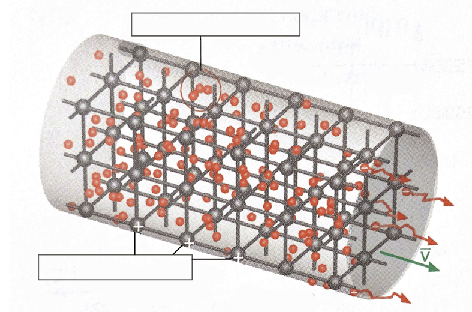
\includegraphics[width=0.6\textwidth]{images/Leiter.png}
    %\caption{Caption}
    \label{fig:Leiter}
\end{figure}

\textbf{Wichtige Begriffe}: Schreiben Sie in Ihren eigenen Worten, was Sie unter diesen Begriffen verstehen.

\vspace{-0.3cm}
\begin{itemize}[label=-]
    \item \textbf{Elektrischer Strom}
	
	\begin{tikzpicture}
		\draw[step=5mm, line width=0.2mm, black!20!white] (0,0) grid  (15.5cm, 2cm);% 10cm);
	\end{tikzpicture}

    \item \textbf{Elektrische Stromstärke} 
	
	\begin{tikzpicture}
		\draw[step=5mm, line width=0.2mm, black!20!white] (0,0) grid  (15.5cm, 2cm);% 10cm);
	\end{tikzpicture}

    \item \textbf{Elektrische Spannung}
	
	\begin{tikzpicture}
		\draw[step=5mm, line width=0.2mm, black!20!white] (0,0) grid  (15.5cm, 2cm);% 10cm);
	\end{tikzpicture}

    \item \textbf{Elektrischer Widerstand}

	\begin{tikzpicture}
		\draw[step=5mm, line width=0.2mm, black!20!white] (0,0) grid  (15.5cm, 2cm);% 10cm);
	\end{tikzpicture}
\end{itemize}


\newpage

\textbf{\large Merkzettel: Stromstärke ($I$) und Spannung ($U$) messen}

\vspace{0.2cm}

\color{red}
\textbf{Wichtig!!!}: Wurde das Messgerät irrtümlich eingestellt, kann die Messschaltung und das Messgerät dabei zerstört werden! Immer \underline{bei ausgeschalteten Spannungsquelle anschliessen} und \underline{doppelt kontrollieren}.
\color{black}

\vspace{0.5cm}

\begin{tcolorbox}[width=\textwidth, %colback=gray!10!white,colframe=gray!75!black]
    colback=white,colframe=gray!75!black]


\textbf{Stromstärke messen}

\vspace{0.2cm}

\begin{wrapfigure}[6]{r}{0.2\textwidth}
\vspace{-12pt}
  \centering
    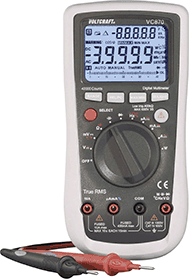
\includegraphics[width=0.15\textwidth]{images/multimeter-vc-870.png}
%    \vspace{-20pt}
  %\caption{\footnotesize text) }
\end{wrapfigure}

\textit{Anschliessen und Einstellen des Messgerätes, oder \textbf{Ampèremeters}}:


Das Gerät muss \textbf{immer mit 2 Kabeln in Serie in den Stromkreis} eingebaut werden („Eingang“ und  „Ausgang“). 
Die beiden Kabel sind an den folgenden Buchsen anzuschliessen: 


\begin{itemize}[label={--}]
    \item „10 A“   (in der Regel rot) / oder Anschluss \underline{nur für geringe Strömstärke}
    \item „COM“  (in der Regel schwarz)
\end{itemize}


Um die Stromstärke korrekt abzulesen, drehen Sie den Drehschalter auf die Stufe ``10 A'' (oder auch ``A'', ``DCA'',  ``A~$\mathdirectcurrent$''  je nach Gerät). Auf dem Display erscheint dann die Stromstärke in der Einheit Ampère. \vspace{0.2cm}

\textit{Hinweis: Wenn in der Anzeige ein Minuszeichen erscheint, können Sie dieses durch Vertauschen der Anschlussbuchsen zum Verschwinden bringen.}

\end{tcolorbox}
\vspace{0.5cm}


\begin{tcolorbox}[width=\textwidth, %colback=gray!10!white,colframe=gray!75!black]
    colback=white,colframe=gray!75!black]

\textbf{Spannung messen}

\vspace{0.2cm}

\begin{wrapfigure}[6]{r}{0.2\textwidth}
\vspace{-12pt}
  \centering
    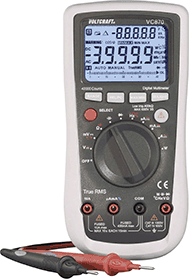
\includegraphics[width=0.15\textwidth]{images/multimeter-vc-870.png}
%    \vspace{-20pt}
  %\caption{\footnotesize text) }
\end{wrapfigure}

\textit{Anschliessen und Einstellen des Messgerätes, oder \textbf{Voltmeters}}:


Das Gerät muss immer mit 2 Kabeln \textbf{parallel} in den Stromkreis eingebaut werden („Eingang“ und  „Ausgang“). 
Die beiden Kabel sind an den folgenden Buchsen anzuschliessen:

\begin{itemize}[label={--}]
    \item „$V\Omega \si{\hertz}CAP$“   (in der Regel rot)
    \item „COM“  (in der Regel schwarz)
\end{itemize}

Um die Spannung abzulesen, drehe den Drehschalter auf die Stufe „$V=$“ (kann je nach Gerät ein wenig unterschiedlich sein). Auf dem Display erscheint dann die Spannung in der Einheit Volt.

%\vspace{0.1cm}

\textit{Hinweis: Wenn in der Anzeige ein Minuszeichen erscheint, können Sie dieses durch Vertauschen der Anschlussbuchsen zum Verschwinden bringen.}
\end{tcolorbox}


\end{document}
